\subsection{Round 1 Problems}

Solutions can be found in Section~\ref{S::2023-S-1}.

\mcq

\begin{enumerate}
    \hyperrefitem[Q::2023-S-1-1] Find the value of $m$ such that $2x^2 + 3x + m$ has a minimum value of 9.
    \begin{tasks}(5)
        \task $\dfrac98$
        \task $-\dfrac98$
        \task $\dfrac{81}8$
        \task $-\dfrac{81}{8}$
        \task $\dfrac{63}{8}$
    \end{tasks}
    \hyperrefitem[Q::2023-S-1-2] Which of the following is true?
    \begin{tasks}(5)
        \task! $\sin{105\deg} - \cos{105}\deg = \dfrac{\sqrt3}{2}$
        \task! $\sin{105\deg} - \cos{105}\deg = \dfrac{\sqrt3}{\sqrt2}$
        \task! $\sin{105\deg} + \cos{105}\deg = \dfrac12$
        \task! $\sin{105\deg} + \cos{105}\deg = \dfrac1{\sqrt3}$
        \task! None of the above
    \end{tasks}
    \hyperrefitem[Q::2023-S-1-3] If $\log_{\sqrt2} x = 10 - 3\log_{\sqrt2} 10$, find $x$.
    \begin{tasks}(5)
        \task 0.32
        \task 0.032
        \task 0.0032
        \task 0.64
        \task 0.064
    \end{tasks}
    \hyperrefitem[Q::2023-S-1-4] If $(x-5)^2 + (y-5)^2 = 5^2$, find the smallest value of $(x+5)^2 + (y+5)^2$.
    \begin{tasks}(5)
        \task! $225 - 100\sqrt2$
        \task! $225 + 100\sqrt2$
        \task! $225\sqrt2$
        \task! $100\sqrt2$
        \task! None of the above
    \end{tasks}
    \hyperrefitem[Q::2023-S-1-5] Suppose $\cos{180\deg + x} = \dfrac45$, where $90\deg < x < 180\deg$. Find $\tan{2x}$.
    \begin{tasks}(5)
        \task $\dfrac{24}{7}$
        \task $\dfrac{7}{24}$
        \task $-\dfrac{24}{7}$
        \task $-\dfrac{7}{24}$
        \task $-\dfrac{24}{25}$
    \end{tasks}
\end{enumerate}

\sq

\begin{enumerate}
    \setcounter{enumi}{5}
    \hyperrefitem[Q::2023-S-1-6] Suppose the roots of $x^2 + 11x + 3 = 0$ are $p$ and $q$, and the roots of $x^2 + Bx - C = 0$ are $p+1$ and $q+1$. Find $C$.
    \hyperrefitem[Q::2023-S-1-7] If the smallest possible value of $(A-x)(23-x)(A+x)(23+x)$ is $-(48)^2$, find the value of $A$ if $A > 0$.
    \hyperrefitem[Q::2023-S-1-8] Find the smallest positive odd integer greater than 1 that is a factor of \[(2023)^{2023} + (2026)^{2026} + (2029)^{2029}.\]
    \hyperrefitem[Q::2023-S-1-9] Find the remainder of $7^{2023} + 9^{2023}$ when divided by 64.
    \hyperrefitem[Q::2023-S-1-10] Let $x, y, z > 1$ and let $A$ be a positive number such that $\log_x A = 30$, $\log_y A = 50$ and $\log_{xy}\bp{Az} = 150$. Find $(\log_A z)^2$.
    \hyperrefitem[Q::2023-S-1-11] Find the largest integer that is less than \[\frac{3^{10} - 2^{10}}{10!} \bp{\frac1{1! 9! 2} + \frac1{2! 8! 2^2} + \frac1{3! 7! 2^3} + \cdots + \frac1{9! 1! 2^9}}^{-1}.\] Here, $n! = n \cdot (n-1) \cdots 3 \cdot 2 \cdot 1$. For example, $5! = 5 \cdot 4 \cdot 3 \cdot 2 \cdot 1 = 120$.
    \hyperrefitem[Q::2023-S-1-12] Consider the following simultaneous equations:
    \begin{align*}
        xy^2 + xyz &= 91\\
        xyz - y^2z &= 72
    \end{align*}
    where $x$, $y$, and $z$ are positive integers. Find the maximum value of $xz$.
    \hyperrefitem[Q::2023-S-1-13] Let $x$ be a real number such that \[\frac{\sin^4 x + \cos^4 x}{\sin^2 x + \cos^4 x} = \frac8{11}.\] Assuming $\sin^2 x > \dfrac12$, find the value of $\sqrt{28} \bp{\sin^4 x - \cos^4 x}$.
    \hyperrefitem[Q::2023-S-1-14] A sequence $a_1, a_2, \ldots$, is defined by \[a_1 = 5, \quad a_2 = 7, \quad a_{n+1} = \frac{a_n + 1}{a_{n-1}} \text{ for $n \geq 2$}.\] Find the value of $100 \times a_{2023}$.
    \hyperrefitem[Q::2023-S-1-15] Let $C$ be a constant such that the equation $5\cos x + 6 \sin x - C = 0$ have two distinct roots $a$ and $b$, where $0 < b < a < \pi$. Find the value of $61 \times \sin{a + b}$.
    \hyperrefitem[Q::2023-S-1-16] In the diagram below, $CE$ is tangent to the circle at point $D$, $AD$ is the diameter of the circle, and $ABC$, $AFE$ are straight lines. It is given that $\frac{AB}{AC} = \frac{16}{41}$ and $\frac{AF}{AE} = \frac{49}{74}$. Let $\tan{\angle CAE} = \frac{m}{n}$, where $m$, $n$ are positive integers and $\frac{m}{n}$ is a fraction in its lowest form. Find the sum $m + n$.

    \begin{center}
        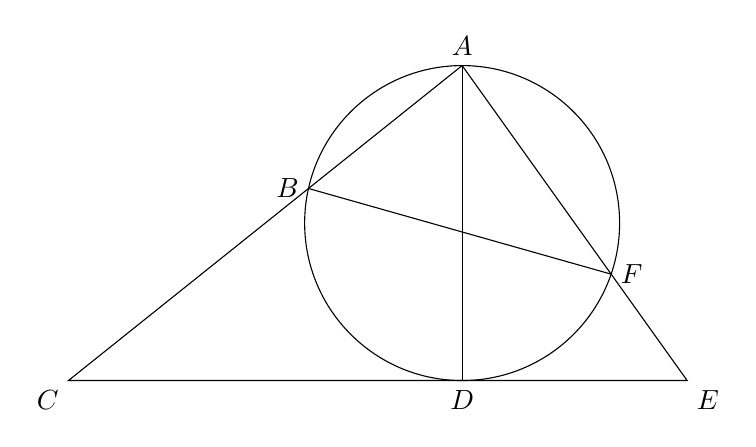
\begin{tikzpicture}[scale=2]
            \coordinate[label=above:$A$] (A) at (0, 1);
            \coordinate[label=left:$B$] (B) at (-40/41, 9/41);
            \coordinate[label=right:$F$] (F) at (35/37, -12/37);
            \coordinate[label=below:$D$] (D) at (0, -1);
            \coordinate[label=below right:$E$] (E) at (1.429, -1);
            \coordinate[label=below left:$C$] (C) at (-2.5, -1);
            
            \draw (0, 0) circle[radius=1];
            \draw (A) -- (E) -- (C) -- (A);
            \draw (A) -- (D);
            \draw (B) -- (F);
        \end{tikzpicture}
    \end{center}
    \hyperrefitem[Q::2023-S-1-17] In the diagram below, $AB$ is a diameter of the circle with centre $O$, $MN$ is a chord of the circle that intersects $AB$ at $P$, $\angle BON$ and $\angle MOA$ are acute angles, $\angle MPA = 45\deg$, $MP = \sqrt{56}$, and $NP = 12$. Find the radius of the circle.

    \begin{center}
        \begin{tikzpicture}[scale=0.6]
            \coordinate[label=above:$A$] (A) at (0, 5);
            \coordinate[label=below:$B$] (B) at (0, -5);
            \coordinate[label=above left:$M$] (M) at (-2.391, 4.391);
            \coordinate[label=below right:$N$] (N) at (4.391, -2.391);
            \coordinate[label=left:$O$] (O) at (0, 0);
            \coordinate[label=above right:$P$] (P) at (0, 2);
    
            \draw (O) circle[radius=5];
            \draw (M) -- (N);
            \draw (A) -- (B);
            
            \fill (P) circle[radius=2.5pt];
            \fill (O) circle[radius=2.5pt];
        \end{tikzpicture}
    \end{center}
    \hyperrefitem[Q::2023-S-1-18] Let $f(x) = \cos[2]{\frac{\pi x}{2}}$. Find the value of \[f\of{\frac1{2023}} + f\of{\frac2{2023}} + \cdots + f\of{\frac{2021}{2023}} + f\of{\frac{2022}{2023}}.\]
    \hyperrefitem[Q::2023-S-1-19] Find the remainder when $3^{2023}$ is divided by 215.
    \hyperrefitem[Q::2023-S-1-20] Find the sum of the prime divisors of 64000027.
    \hyperrefitem[Q::2023-S-1-21] Let $\triangle ABC$ be an equilateral triangle. $D$, $E$, $F$ are points on the sides such that \[BD : DC = CE : EA = AF : FB = 2 : 1.\] Suppose the area of the triangle bounded by $AD$, $BE$ and $CF$ is 2023. Find the area of $\triangle ABC$.

    \begin{center}
        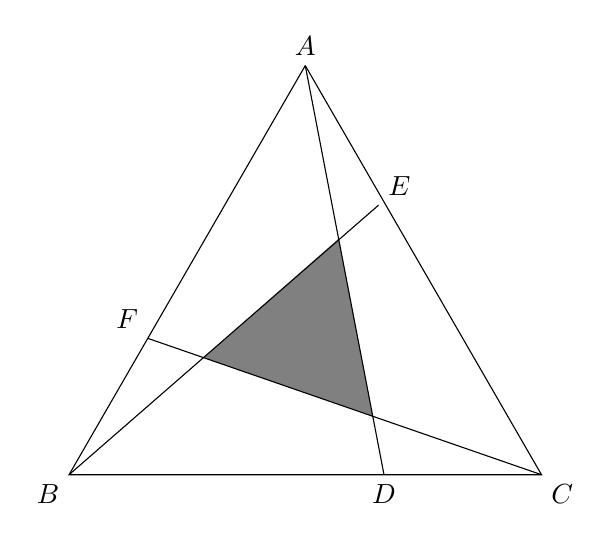
\begin{tikzpicture}[scale=2]
            \coordinate[label=above:$A$] (A) at (0, 2.598);
            \coordinate[label=below left:$B$] (B) at (-1.5, 0);
            \coordinate[label=below right:$C$] (C) at (1.5, 0);
            \coordinate[label=below:$D$] (D) at (0.5, 0);
            \coordinate[label=above right:$E$] (E) at (0.4656, 1.712);
            \coordinate[label=above left:$F$] (F) at (-1, 0.866);
            \coordinate (G) at (0.429, 0.371);
            \coordinate (H) at (0.213, 1.5);
            \coordinate (I) at (-0.646, 0.743);

            \fill[black!50] (G) -- (H) -- (I) -- (G);

            \draw (A) -- (B) -- (C) -- (A);
            \draw (A) -- (D);
            \draw (E) -- (B);
            \draw (C) -- (F);
        \end{tikzpicture}
    \end{center}
    \hyperrefitem[Q::2023-S-1-22] Find the number of possible ways of arranging 10 ones and 11 zeros in a row such that there are in total 13 strings of ones and zeros. For example, \[1110001001110001\] consists of 4 strings of ones and 3 strings of zeros.
    \hyperrefitem[Q::2023-S-1-23] Suppose there exist numbers $a$, $b$, $c$ and a function $f$ such that for any real numbers $x$ and $y$, \[f(x + y) + f(x - y) = 2f(x) + 2f(y) + ax + by + c.\] It is given that \[f(2) = 3, \quad f(3) = -5, \quad \text{ and } \quad f(5) = 7.\] Find the value of $f(123)$.
    \hyperrefitem[Q::2023-S-1-24] Let $f$ be a function such that for any non-zero number $x$, \[6xf(x) + 5x^2 f(1/x) + 10 = 0.\] Find the value of $f(10)$.
    \hyperrefitem[Q::2023-S-1-25] Find the number of triangles such that all the sides are integers and the area equals the perimeter (in number).
\end{enumerate}